\documentclass[../main.tex]{subfiles}

\begin{document}

\subsection{Citations in medical research}

Medical research communication follows a standardised format and occurs primarily through publication \cite{BMCMedicalResearch}. A component of that research is a literature review that contains established facts about a topic. These established facts are corroborated with references to their source of evidence. Citations adhere to a standard format and are typically listed at the end of the research article.

It follows, then, that general information about that research can be elicited from the analysis of these ciations, with the assumption being that studies that cite or are cited by a research article are relevant to that research.

\subsubsection{Improvements in encoder performance using direct citations}

Medical CAL TAR has already benefited from citation utilisation. To date, the most performant encoder model ($BioLinkBERT_{base}$) \cite{yasunaga2022linkbertpretraininglanguagemodels} on the CLEF dataset in a CAL setting leveraged citations between research to achieve state-of-the-art within the CAL process \cite{goharian_reproducibility_2024}. The $LinkBERT$ approach was to view a pertaining corpus as a graph of documents, with each document being a vertex and hyperlinks forming edges between documents. These linked documents were then placed within the same context, which was different from that of $BERT$ random document allocation, in which no linkage between documents within a context window is required. $LinkBERT$ differs from curriculum learning, where a model is provided with examples of increasing difficulty, as the context windows were not ordered by difficulty. A domain-specific variant of $LinkBERT$, $BioLinkBERT$, was created, which was pretrained only on  PubMed articles, with linkage of documents being determined through citations of that research\footnote{https://huggingface.co/michiyasunaga/BioLinkBERT-base}. Models were then trained using standard masked language modelling and next-sentence prediction. The performance of a base model (100M parameters) and a large model (340M parameters) was compared to $PubMedBert$\footnote{https://huggingface.co/microsoft/BiomedNLP-BiomedBERT-base-uncased-abstract-fulltext} in BLURB\cite{guDomainSpecificLanguageModel2021}, MedQA-USMLE\cite{jinWhatDiseaseDoes2020}, and MMLU-professional medicine (medical-specific downstream benchmark tasks)\cite{hendrycksMeasuringMassiveMultitask2021}. $BioLinkBERT_{large}$ achieved state-of-the-art on all reported benchmarks, with an improvement in the BLURB score of 3.2\% above PubMedBERT. 
\begin{figure}[t]
    \centering
    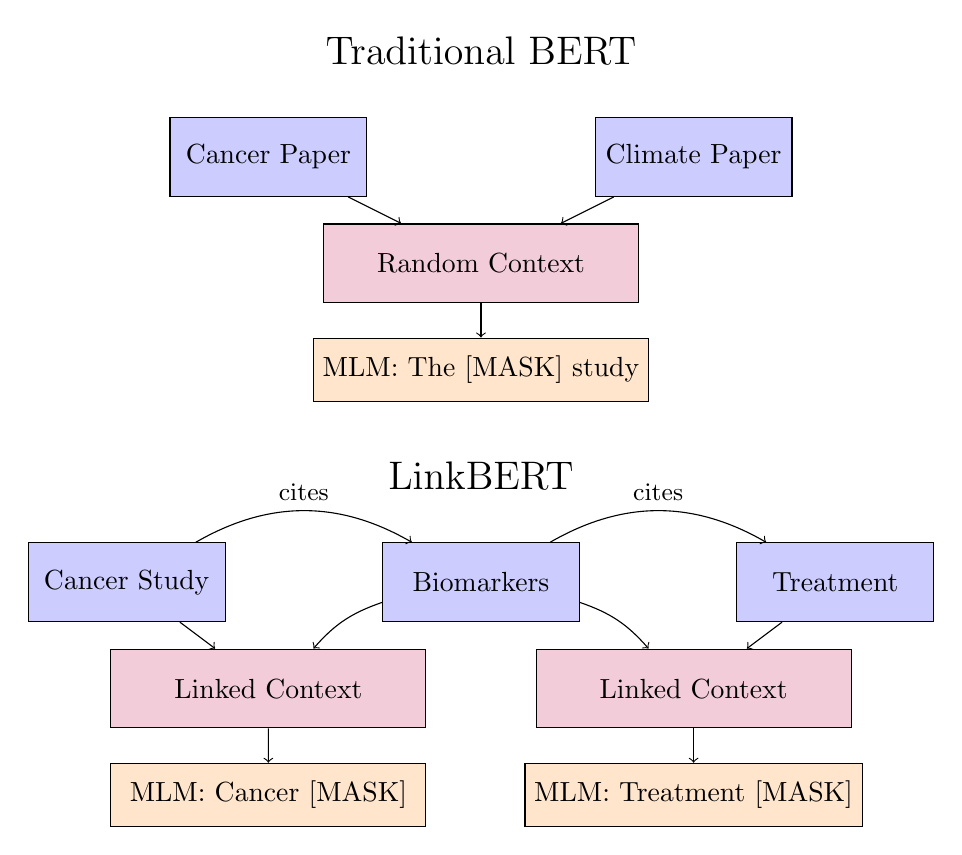
\begin{tikzpicture}[
        doc/.style={rectangle, draw, fill=blue!20, minimum width=2.5cm, minimum height=1cm},
        window/.style={rectangle, draw, fill=purple!20, minimum width=4cm, minimum height=1cm},
        mlm/.style={rectangle, draw, fill=orange!20, minimum width=4cm, minimum height=0.8cm},
        node distance=2cm,
        scale=0.9
    ]
    % Traditional BERT (top)
    \node[align=center] at (-3,5) {\Large Traditional BERT};
    \node[doc] (a1) at (-6,3.5) {Cancer Paper};
    \node[doc] (a2) at (0,3.5) {Climate Paper};
    \node[window] (b1) at (-3,2) {Random Context};
    \node[mlm] (m1) at (-3,0.5) {MLM: The [MASK] study};
    
    \draw[->] (a1) -- (b1);
    \draw[->] (a2) -- (b1);
    \draw[->] (b1) -- (m1);
    
    % LinkBERT (bottom) - with increased horizontal spacing
    \node[align=center] at (-3,-1) {\Large LinkBERT};
    \node[doc] (c1) at (-8,-2.5) {Cancer Study};
    \node[doc] (c2) at (-3,-2.5) {Biomarkers};
    \node[doc] (c3) at (2,-2.5) {Treatment};
    
    \node[window] (d1) at (-6,-4) {Linked Context};
    \node[mlm] (n1) at (-6,-5.5) {MLM: Cancer [MASK]};
    
    \node[window] (d2) at (0,-4) {Linked Context};
    \node[mlm] (n2) at (0,-5.5) {MLM: Treatment [MASK]};
    
    % Citations with curved arrows
    \draw[->, bend angle=30] (c1) to[bend left] node[midway,above] {\small cites} (c2);
    \draw[->, bend angle=30] (c2) to[bend left] node[midway,above] {\small cites} (c3);
    
    % Context connections with slight bends to avoid overlap
    \draw[->] (c1) -- (d1);
    \draw[->] (c2) to[bend right=15] (d1);
    \draw[->] (c2) to[bend left=15] (d2);
    \draw[->] (c3) -- (d2);
    \draw[->] (d1) -- (n1);
    \draw[->] (d2) -- (n2);
    
    \end{tikzpicture}
    \caption{Comparison of document processing in traditional BERT versus LinkBERT. Traditional BERT (top) randomly groups documents into context windows, while LinkBERT (bottom) uses citation relationships to create meaningful document groupings for pre-training. The citation-based grouping ensures that semantically related documents are processed together during masked language modeling tasks.}
    \label{fig:linkbert-comparison}
\end{figure}


In the previously reported Goldilock Reproduce study, in where an Enocder CAL approach was used, $BioLinkBERT_{base}$ formed the classifier. This author recreated their experiment with $BioBERT_{large}$\footnote{https://huggingface.co/michiyasunaga/BioLinkBERT-large} as a classifier model and achieved higher performance in R-Precision in 7 of 12 datasets/policy combinations.  The Friedman test for individual datasets found significant differences between the FPT epochs 4 out of 12 times, however, when considering all datasets together, there was no significant difference between the FPT epochs and R-precision for relancy selection policy or uncertainty selection policy. This indicates that the ``Goldilocks problem'', which was previously reported in the literature in non-medical domains was not apparent when using the large BiolinkBERT model for the CLEF dataset within a CAL process, indicating that further pretraining of models was unneccesary as it does not produce an statistically significant improvement in R-precision. The average R-precision of each FPT epoch is reported in Table \ref{tab:results-average}, with the highest R-precision for relevancy selection policy being 0.847 at further pretrain epoch 2 and the highest R-precision for uncertainty being  0.832 at further pretrain epoch 1. 

Key findings from this research is that an optimal pretraining epoch is unlikely to be found within the CLEF dataset and hence not a viable avenue for future research. In terms of experimental design, certain hyperparameters were chosen without clear reasoning (such as batch size being 25, fine tuning for 20 epochs and stopping after 501 documents labelled). This limitation is thought to be a barrier to improving the performance of the encoder CAL process within that experimental framework, given that reported R-Precision values are already close to the natural ceiling of 1 (with R-Precision reaching 0.945 in some cases). Furturemore, using a more performance/larger model is likely to be fruitful future research, however it is dependent on the availability and development of superior models. This undertaken research did however highlight that leveraging citations themselves was valuable to the CAL process.

A fundamental question emerges from this research: Is contextual understanding of references truly necessary for effective CAL? Several factors suggest that citation networks alone might be sufficient and potentially superior. First, citations themselves represent a form of knowledge distillation, where domain experts have already identified meaningful relationships between documents. Second, analysing reference networks is computationally more efficient than processing full textual contexts. Third, citation network models tend to be more stable when updated, compared to contextual models. Fourth, the contextualization of citation networks may actually introduce noise to what would otherwise be clear citation signals.

While $BioLinkBERT$ represents a sophisticated approach that combines citation networks with contextual language understanding, this integration presents both advantages and limitations. The model's ability to capture complex semantic relationships between documents is valuable, but the contextual processing introduces potential inefficiencies. During pretraining, when linked documents are placed in the same context, the model must process all content within those documents—including sections that may be tangential or unrelated to the citing paper's specific reference. This contextual noise could potentially dilute the precision of the more direct and expertly curated relationships that citations inherently represent. In contrast, pure citation links directly capture intentional scholarly connections made by domain experts, providing a cleaner signal without the additional complexity of processing potentially irrelevant contextual information.
\begin{table}[htbp]
    \centering
    \footnotesize
    \setlength{\tabcolsep}{4pt}
    \begin{tabular}{l>{\raggedright\arraybackslash}p{1.2cm}ccccc}
    \hline
    \textbf{Collection} & \textbf{Dataset size} & \textbf{Model} & \multicolumn{2}{c}{\textbf{R-Precision (↑)}} & \multicolumn{2}{c}{\textbf{Friedman (p)}} \\
    \cline{4-7}
    & & & \textbf{Rel.} & \textbf{Unc.} & \textbf{Rel.} & \textbf{Unc.} \\
    \hline
    \multirow{6}{*}{\makecell[l]{Clef 2019\\dta test}} & 
    \multirow{6}{*}{8} & BiolinkBert-Base-ep0 & \textbf{0.909} & \textbf{0.857} & \multicolumn{2}{c}{---} \\
    & & BiolinkBert-Large-ep0 & 0.897 & 0.803 & \multirow{5}{*}{0.914} & \multirow{5}{*}{0.632} \\
    & & BiolinkBert-Large-ep1 & 0.827 & 0.832 & & \\
    & & BiolinkBert-Large-ep2 & 0.812 & 0.774 & & \\
    & & BiolinkBert-Large-ep5 & 0.841 & 0.814 & & \\
    & & BiolinkBert-Large-ep10 & 0.881 & 0.846 & & \\
    \hline
    \multirow{6}{*}{\makecell[l]{Clef 2017\\test}} & 
    \multirow{6}{*}{30} & BiolinkBert-Base-ep0 & 0.812 & 0.794 & \multicolumn{2}{c}{---} \\
    & & BiolinkBert-Large-ep0 & 0.828 & 0.797 & \multirow{5}{*}{\textbf{\textless0.05}} & \multirow{5}{*}{\textbf{\textless0.05}} \\
    & & BiolinkBert-Large-ep1 & 0.826 & \textbf{0.827} & & \\
    & & BiolinkBert-Large-ep2 & \textbf{0.858} & 0.804 & & \\
    & & BiolinkBert-Large-ep5 & 0.827 & 0.777 & & \\
    & & BiolinkBert-Large-ep10 & 0.799 & 0.757 & & \\
    \hline
    \multirow{6}{*}{\makecell[l]{Clef 2017\\train}} & 
    \multirow{6}{*}{20} & BiolinkBert-Base-ep0 & \textbf{0.838} & 0.761 & \multicolumn{2}{c}{---} \\
    & & BiolinkBert-Large-ep0 & 0.778 & 0.765 & \multirow{5}{*}{\textbf{\textless0.05}} & \multirow{5}{*}{0.28} \\
    & & BiolinkBert-Large-ep1 & 0.808 & 0.789 & & \\
    & & BiolinkBert-Large-ep2 & 0.767 & 0.701 & & \\
    & & BiolinkBert-Large-ep5 & 0.816 & 0.786 & & \\
    & & BiolinkBert-Large-ep10 & 0.827 & \textbf{0.796} & & \\
    \hline
    \multirow{6}{*}{\makecell[l]{Clef 2018\\test}} & 
    \multirow{6}{*}{30} & BiolinkBert-Base-ep0 & 0.794 & 0.780 & \multicolumn{2}{c}{---} \\
    & & BiolinkBert-Large-ep0 & 0.789 & 0.774 & \multirow{5}{*}{0.52} & \multirow{5}{*}{0.50} \\
    & & BiolinkBert-Large-ep1 & \textbf{0.812} & 0.790 & & \\
    & & BiolinkBert-Large-ep2 & 0.797 & \textbf{0.791} & & \\
    & & BiolinkBert-Large-ep5 & 0.763 & 0.773 & & \\
    & & BiolinkBert-Large-ep10 & 0.763 & 0.769 & & \\
    \hline
    \multirow{6}{*}{\makecell[l]{Clef 2019\\DTA int.\\train}} & 
    \multirow{6}{*}{20} & BiolinkBert-Base-ep0 & 0.939 & 0.923 & \multicolumn{2}{c}{---} \\
    & & BiolinkBert-Large-ep0 & 0.939 & 0.902 & \multirow{5}{*}{0.78} & \multirow{5}{*}{0.50} \\
    & & BiolinkBert-Large-ep1 & 0.941 & 0.935 & & \\
    & & BiolinkBert-Large-ep2 & 0.948 & 0.921 & & \\
    & & BiolinkBert-Large-ep5 & 0.952 & 0.945 & & \\
    & & BiolinkBert-Large-ep10 & \textbf{0.945} & \textbf{0.947} & & \\
    \hline
    \multirow{6}{*}{\makecell[l]{Clef 2019\\DTA int.\\test}} & 
    \multirow{6}{*}{20} & BiolinkBert-Base-ep0 & \textbf{0.934} & \textbf{0.900} & \multicolumn{2}{c}{---} \\
    & & BiolinkBert-Large-ep0 & 0.899 & 0.856 & \multirow{5}{*}{0.87} & \multirow{5}{*}{\textbf{\textless0.05}} \\
    & & BiolinkBert-Large-ep1 & 0.904 & 0.840 & & \\
    & & BiolinkBert-Large-ep2 & 0.909 & 0.878 & & \\
    & & BiolinkBert-Large-ep5 & 0.882 & 0.835 & & \\
    & & BiolinkBert-Large-ep10 & 0.865 & 0.841 & & \\
    \hline
   
    \end{tabular}
    \caption{Performance comparison across different collections and models}
    \label{tab:results}
\end{table}

\begin{table}[htbp]
    \centering
    \caption{Average R-precision of each FPT epoch for CLEF dataset}
    \begin{tabular}{l>{\raggedright\arraybackslash}p{1.2cm}ccccc}
        \textbf{Policy} & \textbf{ep0} & \textbf{ep1} & \textbf{ep2} & \textbf{ep5} & \textbf{ep10} \\
        \hline
        Uncertainty & 0.813 & 0.832 & 0.813 & 0.815 & 0.814 \\
        Relevancy & 0.840 & 0.845 & 0.847 & 0.842 & 0.835 \\
    \hline

    \end{tabular}
    \label{tab:results-average}
\end{table}



\subsubsection{Direct citation network mining within medicine research}

Despite these more complex citation network mining approaches being somewhat performant, simpler, more robust approaches to citation network mining already exist within medicial research. Let G be a citation graph where:

\begin{itemize}
    \item $D_i$ represents a research article of interest as a vertex in G
    \item $D_{ip}$ represents the set of articles referenced by $D_i$
    \item $D_{if}$ represents the set of articles that reference $D_i$
    \item Both sets are subsets of G: $D_{ip}, D_{if} \subset G$
    \item $D_{ip} \cap D_{if} = \emptyset$, so searching both sets will provide different relevant articles
\end{itemize}

Relevancy is defined as a function $R: D \rightarrow [0,1]$, where:

\begin{itemize}
    \item 0 denotes no relevance
    \item 1 denotes maximum relevance
    \item For any set of documents $D_{set}$, relevancy is defined as $R(D_{set}) = {R(d) | d \in D_{set}}$
\end{itemize}

Two primary search approaches are defined:
\begin{itemize}
    \item Backward citation searching (BCS): examining all articles in $D_{ip}$\cite{lefebvre2011cochrane, akers2009systematic}
    \item Forward citation searching (FCS): examining all articles in $D_{if}$*\footnote{FCS involves using a citation index to identify studies that cite a source study. A citation index is a database of scholarly articles and their citations, such as PubMed, Google Scholar, Scopus or OpenAlex}
\end{itemize}

These approaches are both simple and effective, inherently respecting temporal relationships between research articles (i.e., you cannot cite a paper that has yet to be published). More so, BCS and FCS are recommended to be used in the identification phase of cochrane systematic review generation, with 87\% of cochrane reviews between November 2016 to January 2017 reporting the use of BCS and 9\% reporting the use of FCS\cite{briscoeConductReportingCitation2019}. Recommendations regarding BCS/FCS in the the search stage are found within the Cochrane Handbook, with BCS being mandatory (C30), and FCS not being mentioned \cite{MECIRManualCochrane}. No such recommendations exist for BCS and FCS use within the screening phase within the Cochrane Handbook. 
Additionally, there is a paucity of research outlining the use of BCS and FCS within the active learning process when searching multiple citation indexes (Search Strategy outlined in Figure \ref{fig:search-results}). An important clarification is required to understand the novality of this approach. As previously mentioned, this PhD is focusing on the title and abstract screening phase within the screening phase of systematic review generation. BCS and FCS is traditionally used in the identification phase only \ref{fig:selection_and_screening}, with title and abstracts being screened to reduce the work required in the more costly full text screening phase. This is not a limiting factor for comptuation, and hence restriction of this phase to just title and abstracts is redundant. This amendment to the screening process is also not intended to remove the full text screening phase, as each phase has a different requirement, with title and abstract screening being focused only on relevancy to the topic, and full text screening being focused on quality and eligibility of the research.

\begin{figure}[htbp]
    \centering
    \begin{tikzpicture}[
        node distance = 0.5cm,
        box/.style={rectangle, draw, text width=4cm, minimum height=1cm, align=center},
        query/.style={rectangle, draw, fill=gray!10, text width=4cm, minimum height=2.5cm, align=center}
    ]
        % Search queries side by side
        \node[query] (q1) {Search Query 1:\\
            (``backward citation'' OR\\``citation analysis'')\\
            AND ``active learning''};
        \node[query] (q2) [right=0.5cm of q1] {Search Query 2:\\
            (``citation graph'' OR\\``citation network'') AND\\(``active learning'' OR\\``interactive learning'')};
        \node[query] (q3) [right=0.5cm of q2] {Search Query 3:\\
            (``bibliometric analysis'' OR\\``reference mining'') AND\\(``selective sampling'' OR\\``query learning'')};
            
        % Results box below
        \node[box] (results) [below=1cm of q2] {No Related Documents Found};
            
        % Arrows
        \draw[-stealth] (q1) -- (results);
        \draw[-stealth] (q2) -- (results);
        \draw[-stealth] (q3) -- (results);
        
    \end{tikzpicture}
    \caption{Results from literature search on citation index arxiv and pubmed demonstrating absence of related works, ran on 13th November 2024}
    \label{fig:search-results}
\end{figure}
\begin{center}
\begin{tikzpicture}[
    > = {Stealth[scale=1.2]},
    vertex/.style = {circle, draw, minimum size=1.2cm, inner sep=1pt},
    ref_edge/.style = {->, thick, blue},
    label_style/.style = {font=\small}
]

% Main document Di
\node[vertex, fill=yellow!20] (Di) at (0,0) {$D_i$};

% Past references (Dip) - More fanned out
\node[vertex] (Dip1) at (-3,2.5) {$D_{ip1}$};
\node[vertex] (Dip2) at (0,3) {$D_{ip2}$};
\node[vertex] (Dip3) at (3,2.5) {$D_{ip3}$};

% Future references (Dif) - More fanned out
\node[vertex] (Dif1) at (-3,-2.5) {$D_{if1}$};
\node[vertex] (Dif2) at (0,-3) {$D_{if2}$};
\node[vertex] (Dif3) at (3,-2.5) {$D_{if3}$};

% Edges for past references
\draw[ref_edge] (Di) -- (Dip1);
\draw[ref_edge] (Di) -- (Dip2);
\draw[ref_edge] (Di) -- (Dip3);

% Edges for future references
\draw[ref_edge] (Dif1) -- (Di);
\draw[ref_edge] (Dif2) -- (Di);
\draw[ref_edge] (Dif3) -- (Di);

% Labels for sets
% \node[label_style] at (-4,2) {$D_{ip}$ (Referenced by $D_i$)};
% \node[label_style] at (-4,-2) {$D_{if}$ (References to $D_i$)};

% Relevancy function examples
\node[label_style] at (5,2.5) {$R(D_{ip1}) = 0.8$};
\node[label_style] at (5,2) {$R(D_{ip2}) = 0.3$};
\node[label_style] at (5,1.5) {$R(D_{ip3}) = 0.5$};
\node[label_style] at (5,-1.5) {$R(D_{if1}) = 0.6$};
\node[label_style] at (5,-2) {$R(D_{if2}) = 0.4$};
\node[label_style] at (5,-2.5) {$R(D_{if3}) = 0.9$};

% Time arrow (vertical)
\draw[{Stealth[scale=1.5]}->, thick] (7,3.5) -- (7,-3.5);
\node[label_style] at (7,3.8) {Past};
\node[label_style] at (7,-3.8) {Future};

\end{tikzpicture}
\end{center}

While the citation network mining approach could be used to group articles of interest within a context window, similar to that of $BioLinkBERT$ (which used FCS, and not BCS), pretraining a model from scratch using this approach is obviously outside the possibility of this PhD project, due to hardware constraints. Citation network mining can however be used to augment the CAL process in ways that overcome some of the limitatitions of this process. 

Firstly, CAL requires labelled data to train the classifier model, with the more data being available, with the assumption that the better the model is expected to perform. Encoder CAL approaches suffer disproportionately to that of feature-based CAL approaches due to their need for larger amounts of training data to effectively learn meaningful representations. This is because encoder models like BERT need to learn complex contextual relationships between words and concepts, whereas feature-based models can rely on simpler statistical patterns. When working with limited labeled data in the early stages of screening, encoder models may struggle to generalize well, potentially leading to suboptimal performance in identifying relevant documents. As discussed in the Encoder CAL process, often a single sample seed document is used during the first epoch for fine-tuning. A better approach would be to exhaust the citation network of that seed document first for labelling, before using revealed relevant documents to fine-tune the model, potentially resulting in a more performant model at the earlier stages of screening with less oracle cost. This potentially overcomes limitations of the Encoder CAL process, and also reduces computational costs (as citation network mining is less computationally expensive than fine-tuning). 

Early work performed by the Author on a subset of the CLEF dataset demonstrates that exhausting the BCS network of a seed document resulted in greater R-Precision values when compared to that of the Encoder CAL process at similar points. The logical, and simple augmentation of the encoder CAL approach would be to exhaust both BCS and FCS networks of a seed document prior to initiating the encoder CAL process. This 
\subsubsection{More advanced citation network mining}

One of the issues with citation network mining is that it is not able to identify indirect citations. For example, if $D_i$ references $D_{ip1}$ and $D_{ip1}$ references $D_{ip2}$, then $D_i$ and $D_{ip2}$ are related, even though $D_i$ does not cite $D_{ip2}$ directly. This limitation would prevent the use of citation network mining to replace the encoder CAL process entirely. Other citation network mining approaches have been proposed to address this issue:


\begin{center}
    \begin{tikzpicture}[
        > = {Stealth[scale=1.2]},
        vertex/.style = {circle, draw, minimum size=1.2cm, inner sep=1pt},
        ref_edge/.style = {->, thick, blue},
        indirect_edge/.style = {->, thick, red, dashed},
        label_style/.style = {font=\small}
    ]
    
    % Main document Di
    \node[vertex, fill=yellow!20] (Di) at (0,0) {$D_i$};
    
    % Direct reference
    \node[vertex] (Dip1) at (-2,2) {$D_{ip1}$};
    
    % Indirect reference
    \node[vertex] (Dip2) at (2,4) {$D_{ip2}$};
    
    % Add edges
    \draw[ref_edge] (Di) -- (Dip1) node[midway, left] {Direct};
    \draw[ref_edge] (Dip1) -- (Dip2) node[midway, right] {Direct};
    \draw[indirect_edge] (Di) to[bend right] node[midway, right] {Indirect} (Dip2);
    
    % Time arrow (vertical)
    \draw[{Stealth[scale=1.5]}->, thick] (4,4.5) -- (4,-1);
    \node[label_style] at (4,4.8) {Past};
    \node[label_style] at (4,-1.3) {Future};
    
    % Legend
    \node[label_style] at (6,2) {Legend:};
    \draw[ref_edge] (5,1.5) -- (7,1.5) node[right] {Direct citation};
    \draw[indirect_edge] (5,1) -- (7,1) node[right] {Indirect citation};
    
    \end{tikzpicture}
    \end{center}
\end{document}



